\documentclass[thesis.tex]{subfiles}
\begin{document}

\chapter{Einleitung}
\label{chap:Einleitung}

% An image right here at the top can look really cool!
\begin{figure}[h]
    \centering
    % 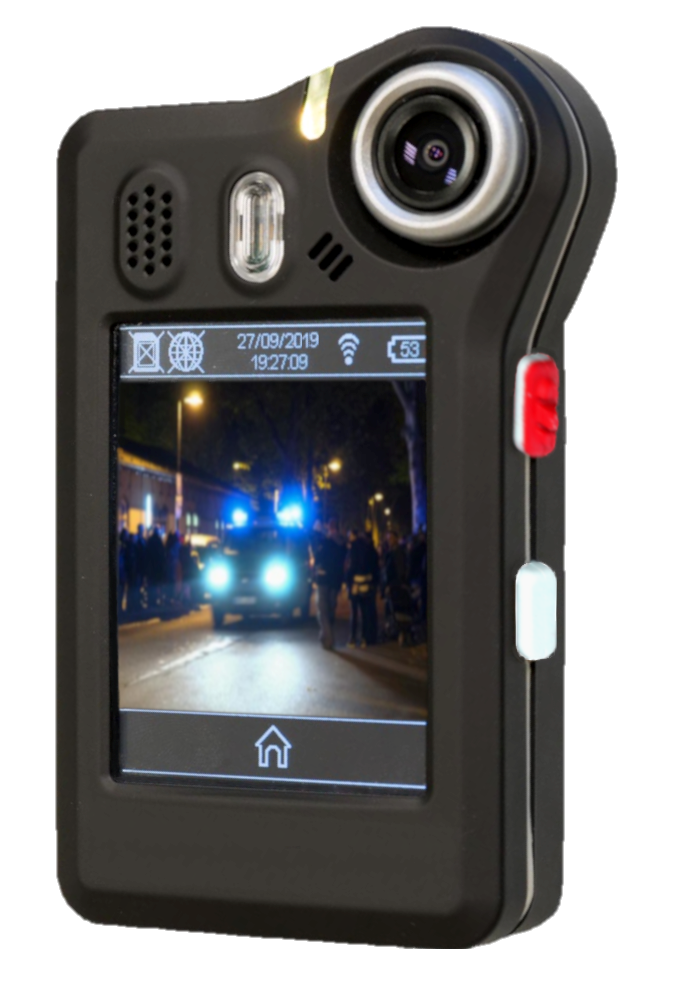
\includegraphics[height=0.5\textwidth]{/BC_activDisplay.png}
    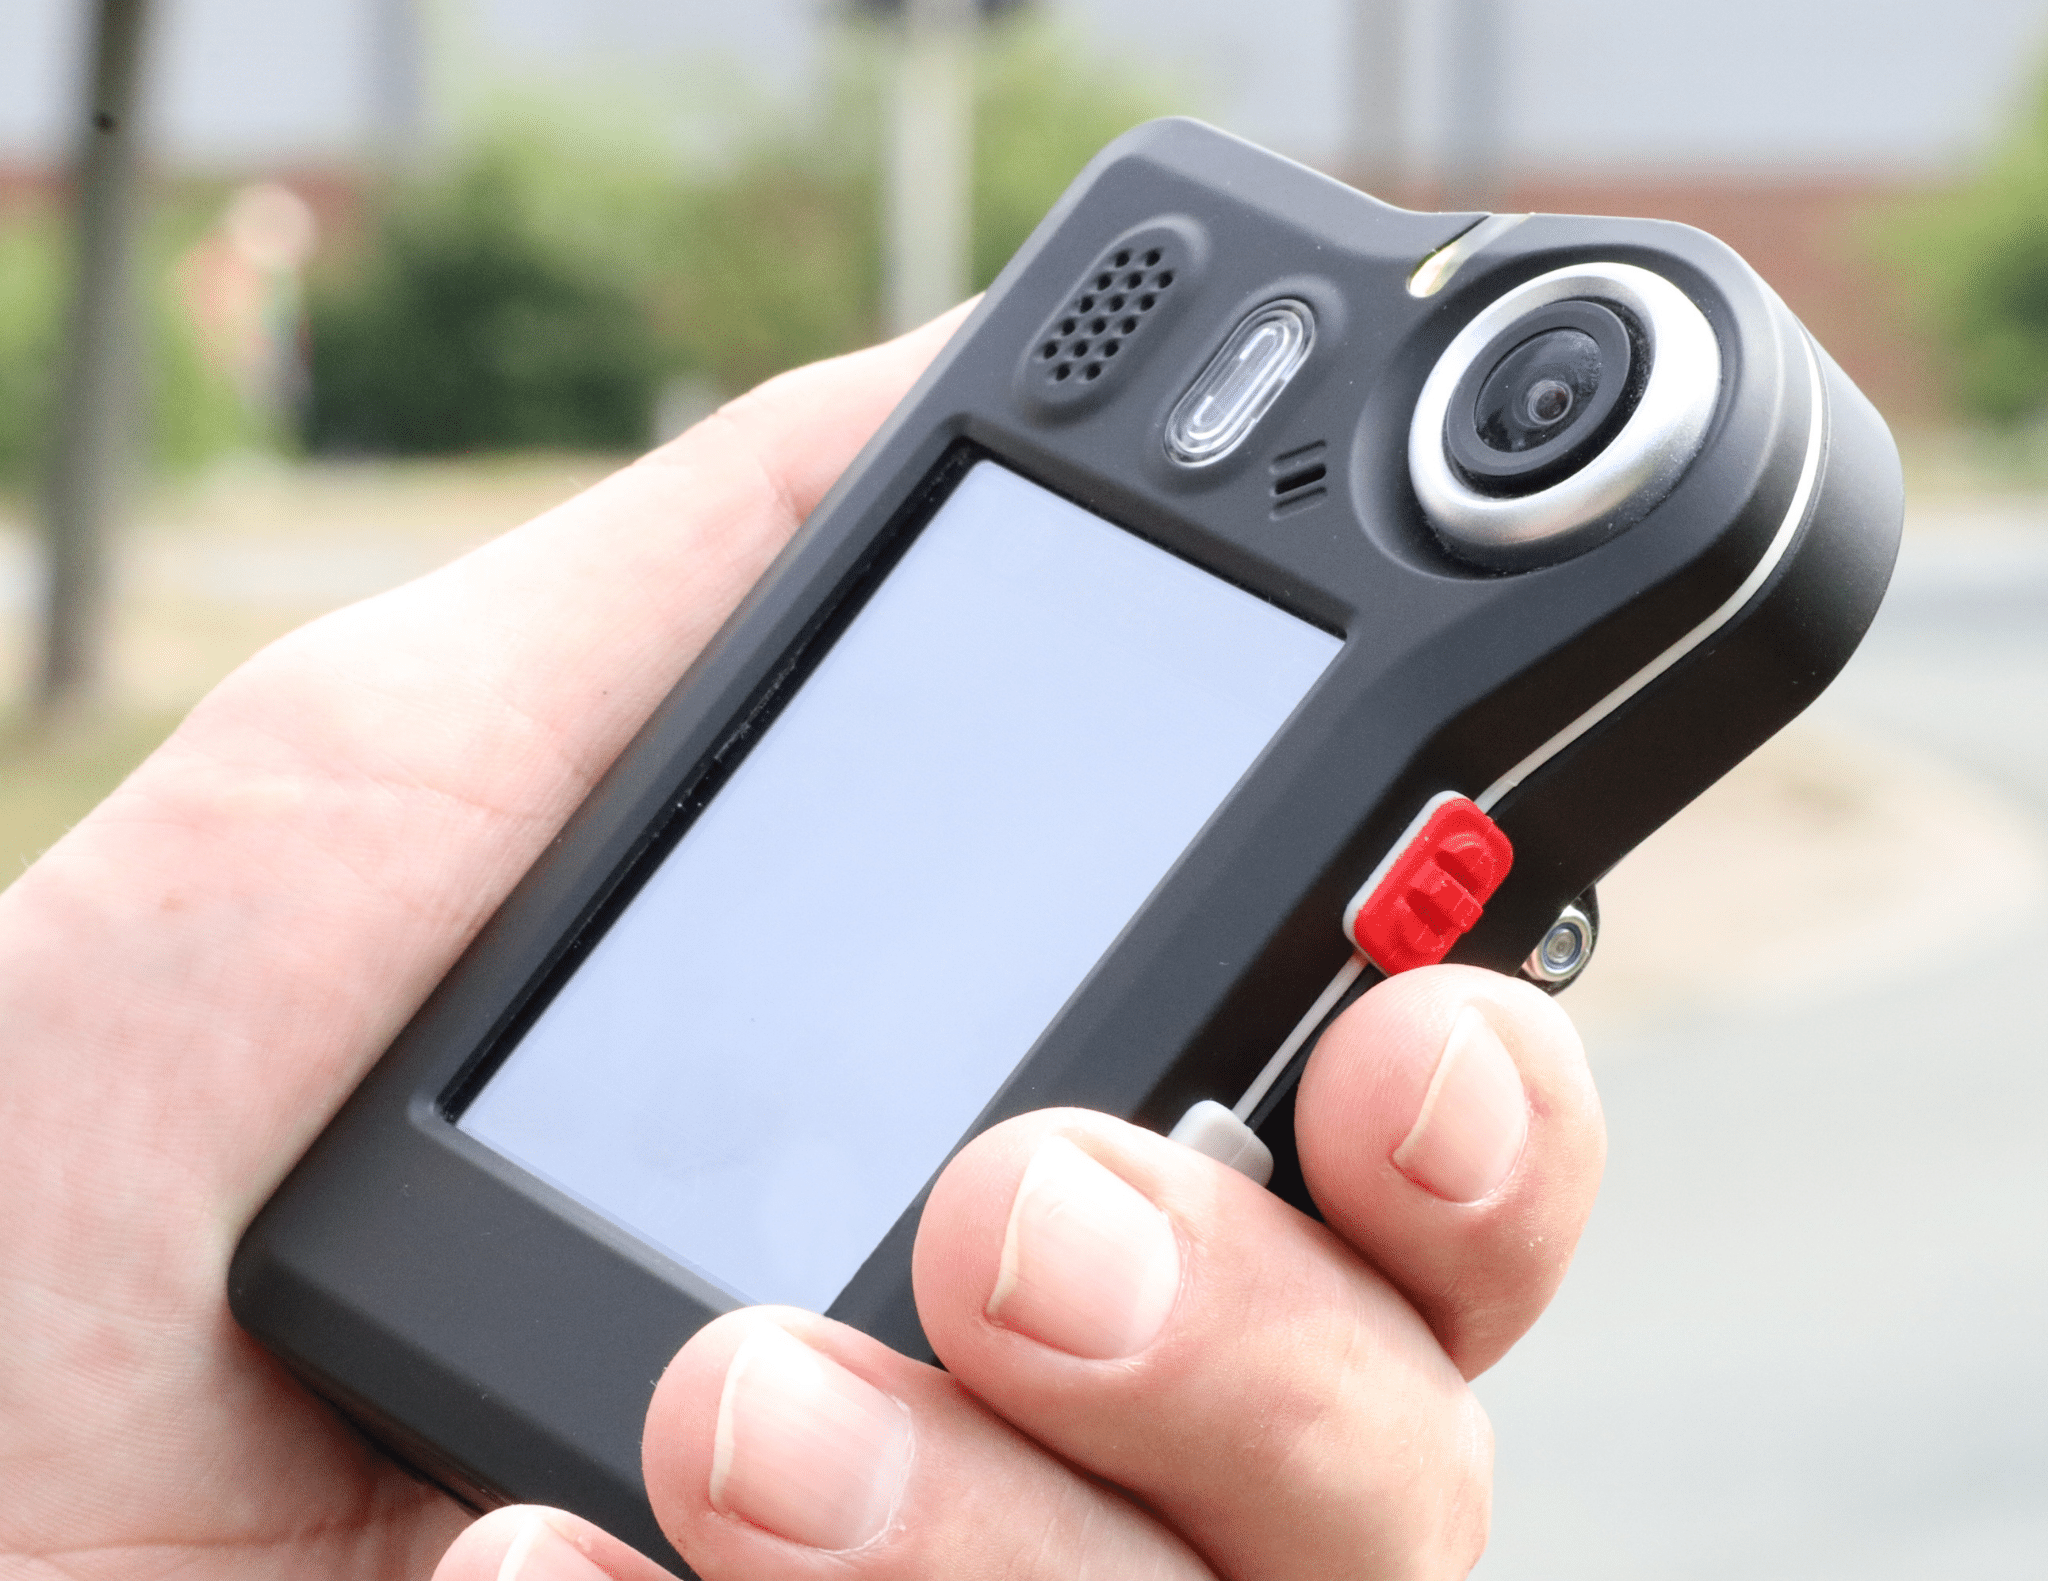
\includegraphics[height=0.55\textwidth]{/BC_hand.png}
    \caption{NetCo Body-Cam}
    \label{fig:BC}
\end{figure}

Das Unternehmen NetCo Professional Services GmbH mit Sitz in Blankenburg und Magdeburg entwickelt und produziert individuelle Kamera- und Softwarelösungen.
Ein Hauptprodukt, die NetCo Body-Cam (BC), wurde 2016 im Auftrag eines englischen Partners entwickelt, für den deutschen Markt angepasst und wird inzwischen europaweit erfolgreich vertrieben.
Sie dient gegenwärtig in erster Linie zur Prävention und Deeskalation bei Konflikten in den Einsatzszenarien von Polizei, Ordnungsämtern, Verkehrsbetrieben und Sicherheitsdiensten, sowie zur deren Dokumentation, im Speziellen zur rechtskonformen Beweissicherung und deren Gerichtsverwertbarkeit.

Prävention und Deeskalation sind vor allem im Bereich Arbeitsschutz bzw., bei der Verhinderung von Arbeitsunfällen ein wichtiges Thema.
In Bahnbetrieben, zum Beispiel, fallen im Jahr 2020 knapp 27 \% und im Jahr 2021 über 21 \% aller Arbeitsunfälle in die Kategorie "Einwirkungen durch Gewalt, Angriff, Bedrohung", davon über 60 \% durch betriebsfremde Personen, also z.B. Fahrgäste \cite[jeweils S.87 ff.]{Unfallgeschehen2020,Unfallgeschehen2021}.
Ob die abnehmende Tendenz mit dem Einsatz der Bodycams erklärt werden kann, ist noch nicht hinreichend evaluiert, lässt jedoch positive Auswirkungen annehmen.
Die NetCo Body -Cam wird gegenwärtig in zwei Versionen angeboten.
In der Record-Version wird die Aufnahme im Gerät gespeichert und nach dem Einsatz über eine Docking-Station in das zentrale System überspielt.
In der Connect-Version erfolgt die unmittelbare Übertragung über VPN an das zentrale System.
Beide Systemvarianten decken die Zielstellungen Prävention, Deeskalation und Dokumentation zuverlässig ab.

Durch verstärkte Kundenanfragen lassen sich zunehmend weitere Zielstellungen und damit Einsatzgebiete identifizieren.
So nimmt die Absicherung von Alleinarbeitern einen immer größeren Stellenwert ein.

Alleinarbeit (engl. Lonework) wird nach (DGVU §8) \cite[§8]{Vorschrift1_DGUV} unter bestimmten Umständen als gefährliche Arbeit eingestuft, z.B. Dienstleistungen an Personen, die sich gegen die Dienstleistung tätlich wehren, wie es in der mobilen Pflege, den Verkehrsbetrieben oder in der speziellen Jugendhilfe der Fall sein kann.
Unter 2.7.2 DGVU-Regel 100-001 "Regeln zur Prävention" heißt es: "Wird eine gefährliche Arbeit von einer Person allein ausgeführt, so hat der Unternehmer über die allgemeinen Schutzmaßnahmen hinaus für geeignete technische oder organisatorische Personenschutzmaßnahmen zu sorgen \cite[§8(2)]{Vorschrift1_DGUV}.
Alleinarbeit liegt vor, wenn eine Person allein, außerhalb von Ruf- und Sichtweite zu anderen Personen, Arbeiten ausführt" \cite[S.42]{Regel_100-001}.
Nach Geyer \& Magiera folgt diese Fürsorge einem gesetzlich geregeltem Schema aus den Bausteinen: Festlegung der Arbeitsbereiche und Tätigkeiten, Ermittlung der Gefährdungen und Festlegung konkreter Arbeitsschutzmaßnahmen, inklusive Umsetzung, sowie Wirkungskontrolle \cite[vgl. S.42 ff.]{GeyerMagiera2022}.
Wird erhöhte oder kritische Gefährdung ermittelt, erfordert es Schutzmaßnahmen durch Überwachung in unterschiedlicher Ausprägung.

In dieser notwendigen Weiterentwicklung unseres Produktes soll die BC für spezielle Einsatzzwecke nun den sogenannten Lone-Worker-Modus als neues Feature bekommen.
Durch diesen Modus soll die Sicherheit des Trägers durch erweiterte Notrufmöglichkeiten im Notfall im Fokus stehen.
Weiterhin bietet die BC eine als entlastend empfundene mentale Unterstützung durch die geeignete Überwachung.
Nach Geyer \& Magiera ergeben sich neben den häufig ersichtlichen Gefährdungsfaktoren durch Arbeitsumgebungsbedingungen weitere Einflüsse auf die Beurteilung der Gefährdungen im Zusammenhang mit Alleinarbeit.
Unter anderem ist zu fragen, wie Alleinarbeit auf den Mitarbeitenden in Summe wirkt.
Dabei ist auch an psychische Belastungen durch Alleinarbeit zu denken, z. B.: die Vorstellung bzw. Angst, dass niemand zu Hilfe kommt, wenn etwas passiert, Stress wegen mangelnder Unterstützung bei außergewöhnlichen Ereignissen oder das Gefühl der Isolation \cite[vgl. S.45]{GeyerMagiera2022}.

Für dieses Wirkspektrum wird eine kontinuierliche Verbindung mit einer Überwachungszentrale bereitgestellt.
So können einerseits Sicherheit vermittelt werden und andererseits unerwartete Situationen erkannt und schnell reagiert werden.
Um die Verbindung und die damit verbundene Sicherheit festzustellen, müssen beide Seiten in kurzer Zeit einen Verbindungsverlust erkennen und nach vorher definierten Handlungen reagieren, wie z.B. das Auslösen eines Alarms.
Damit einhergehend müssen Prozeduren geschaffen werden, die einen sauberen und sicheren Übergang von aktivem und inaktivem Modus sicherstellen und diesen von einem unerwarteten Verbindungsverlust abgrenzen können.
Außerdem sollte bei einem plötzlichen Verbindungsabbruch die Kommunikation so schnell wie möglich und automatisch wieder hergestellt werden.
Dies stellen Mobilfunk oder WLAN nativ nicht zur Verfügung.
Neben den vorhandenen Funktionen der Body-Cam (Aufnahme, Streaming, Dokumentation), sollen durch den LW-Modus weitere Optionen geschaffen werden.
Diese sollen sicherstellen, dass die Body-Cam alle nötigen Voraussetzungen erfüllt, um die Sicherheit einer allein arbeitenden Person zu unterstützen.
Darunter zählen beispielsweise Alarmsignalisierung, Geräteüberwachung, Sprachkommunikation, Video- und Audiostreaming, Textnachrichten oder Geofencing.
Alle Ereignisse muss die Body-Cam sicher und nachvollziehbar protokollieren.

Die vorliegende Bachelorarbeit gliedert sich in drei Hauptteile.
Im ersten Teil werden die Grundlagen für die weitere Arbeit gelegt.
Dazu wird beschrieben was Alleinarbeit ist und wie sich diese in verschiedene Gefährdungsstufen einteilen lässt.
Außerdem welche aktuellen Alleinarbeitslösungen es gibt und wie sich die Body-Cam mit dem LW-Modus dort einordnen lässt.
Anschließend wird der aktuelle Zustand der Body-Cam aufgezeigt und beschrieben wie diese durch die neue Lone-Worker Funktion erweitert wird.
Weiterhin wird das sich daraus ergebene Gesamtsystem beschrieben und dessen Anforderungen herausgearbeitet.
Diese ergeben sich aus den DGUV-Normen und zusätzlichen Unternehmensanforderungen.
Im zweiten Teil wird das Designkonzept behandelt.
Dafür werden aus den Anforderungen die verschiedenen Funktionen erarbeitet, die in den LW-Modus der Body-Cam einfließen.
Des Weiteren wird das Protokoll und dessen Aufbau erläutert um eine Kommunikation zwischen der Body-Cam und dem Überwachungszentrum sicherzustellen.
Außerdem werden alle Schnittstellen beschrieben die sich zwischen der bestehenden Body-Cam Implementierung und dem neuen Lonewoker-Modus ergeben.
Zusätzlich wird durch Statusmaschinen die Implementierung der Funktionen in ein einfaches Schema gebracht und die Realisierung damit vorbereitet.
Der letzte Teil behandelt die Realisierung des Projekts.
Hier werden zuerst die verwendeten Technologien und technischen Grundlagen erklärt.
Danach folgt die Implementierung, in dem der Entwicklungsprozess beschrieben wird, um auf Herausforderungen einzugehen.
Anschließend wird der zuvor entwickelte Prototyp durch ein Testprotokoll auf seine Funktion überprüft und die Ergebnisse werden ausgewertet.


% \autoref{chap:grundlagen} discusses ...
% \\
% Our own contribution ... described in \autoref{chap:design}.
% Results are evaluated and discussed in \autoref{chap:ergebnisse}.
% \\
% Finally, \autoref{chap:fazit} will summarize the thesis and give an outlook to possible future work.

\subfilebib % Makes bibliography available when compiling as subfile
\end{document}